% Usage: knitr slide

\chapter{Comparing Two Proportions} \ros{10.1-10.3, 10.5}\katz{5.2}

\section{Overview}

\bi
 \item Compare dichotomous independent variable with a dichotomous outcome
  \bi
  \item Independent variables: Exposed/Not, Treatment/Control, Knockout/Wild Type, etc.
  \item Outcome (dependent) variables: Diseased/Not or any Yes/No outcome 
  \ei
 \item Continuous outcomes often dichotomized for analysis (bad idea)
  \bi
  \item Consider $t$-tests (Chapter 3) or Non-parameteric methods (Chaper 5)
  \ei
\ei

\section{Normal-Theory Test}
\bi
\item Two independent samples

%, sizes $n_{1}, n_{2}$
%\item Unknown population probabilities of event $p_{1}, p_{2}$
%\item Sample proportions for estimating $p_{1},p_{2}$: $\hat{p}_{1},
%  \hat{p}_{2}$
\begin{tabular}{lcc} 
 & \underline{Sample 1} & \underline{Sample 2} \\
Sample size & $n_1$ & $n_2$ \\
Population probability of event & $p_1$ & $p_2$ \\
Sample probability of event & $\hat{p}_1$ & $\hat{p}_2$ \\
\end{tabular}

\item Null Hypothesis, $H_{0}: p_{1}=p_{2}=p$
\item Estimating the variance
\bi 
 \item Variance of $\hat{p}_{i} = p_{i}(1-p_{i})/n_{i}$ for $i = 1, 2$
 \item Variance of $\left(\hat{p}_1 - \hat{p}_2\right)$ is the sum of the
  variances, which under $H_{0}$ is
   \beq
    p(1-p)[\frac{1}{n_{1}}+\frac{1}{n_{2}}]
   \eeq
 \item We estimate this variance by plugging $\hat{p}$ into $p$, where
 \beq
 \hat{p} = \frac{n_{1}\hat{p}_{1}+n_{2}\hat{p}_{2}}{n_{1}+n_{2}}
 \eeq
 is the pooled estimate of the probability under $H_{0}: p_1 = p_2 = p$
\ei
\item Test statistic which has approximately a normal distribution
  under $H_{0}$ if $n_{i}\hat{p}_{i}$ are each large enough:
\beq
z = \frac{\hat{p}_{1} -
  \hat{p}_{2}}{\sqrt{\hat{p}(1-\hat{p})[\frac{1}{n_{1}}+\frac{1}{n_{2}}]}}
\eeq
\item To test $H_{0}$ we see how likely it is to obtain a $z$ value as
  far or farther out in the tails of the normal distribution than $z$
  is
\item We don't recommend using the continuity correction
\item Example:  \\
Test whether the population of women whose age at first birth $\leq
29$ has the same probability of breast cancer as women whose age at
first birth was $\geq 30$.  This dichotomization is highly arbitrary
and we should really be testing for an association between age and
cancer incidence, treating age as a continuous variable.
\item Case-control study (independent and dependent variables
  interchanged); $p_{1}=$ probability of age at first birth $\geq 30$,
  etc.

\begin{tabular}{lcc} 
 & \underline{with Cancer} & \underline{without Cancer} \\
Total \# of subjects & $3220 (n_1)$ & $10245 (n_2)$ \\
\# age $\geq 30$ & $683$ & $1498$ \\ \\
Sample probabilities & $0.212 (\hat{p}_1$) & $0.146 (\hat{p}_2$) \\ \\
Pooled probability &\multicolumn{2}{c}{$\frac{683 + 1498}{3220 + 10245} = 0.162$} \\
\end{tabular}


%\beqa
%n_{1}=3220, n_{2}=10245, \\ 
%\hat{p}_{1}=\frac{683}{3220}=0.212, \\
%\hat{p}_{2}=\frac{1498}{10245} = 0.146 \\
%\hat{p}=\frac{683+1498}{3220+10245} = 0.162 \\
\item Estimate the variance
  \bi
  \item $\mathrm{variance}(\hat{p}_{1}-\hat{p}_{2}) = \hat{p}(1-\hat{p})\times \left[\frac{1}{n_{1}}+\frac{1}{n_{2}}\right] = 5.54 \times 10^{-5}$ \\
  \item $SE = \sqrt{\mathrm{variance}} = 0.00744$ \\
  \ei
\item Test statistic
  \bi 
  \item $z = \frac{0.212-0.146}{0.00744} = 8.85$
  \ei
\item 2-tailed $P$-value is $ < 10^{-4}$
\begin{Schunk}
\begin{Sinput}
n1 <- 3220;     n2 <- 10245
p1 <- 683 / n1; p2 <- 1498 / n2
pp <- (n1 * p1 + n2 * p2) / (n1 + n2)
se <- sqrt(pp * (1 - pp) * (1 / n1 + 1 / n2))
z  <- (p1 - p2) / se
pval <- 2 * (1 - pnorm(abs(z)))
round(c(p1=p1, p2=p2, pooled=pp, se=se, z=z, pval=pval), 4)
\end{Sinput}
\begin{Soutput}
    p1     p2 pooled     se      z   pval 
0.2121 0.1462 0.1620 0.0074 8.8527 0.0000 
\end{Soutput}
\end{Schunk}
\item We do not use a $t$-distribution because there is no $\sigma$ to
  estimate (and hence no ``denominator d.f.'' to subtract)
\ei

\section{$\chi^2$ Test}
\bi
\item If $z$ has a normal distribution, $z^2$ has a $\chi^2$
  distribution with 1 d.f. (are testing a single difference against zero)
\item The data we just tested can be shown as a $2\times 2$
  contingency table

\begin{tabular}{l|c|c|c} 
\multicolumn{1}{l}{} & \multicolumn{1}{c}{Cancer +} & \multicolumn{1}{l}{Cancer -} \\ \cline{2-3}
Age $\leq 29$ & $2537 $ & $8747$ & $11284$ \\ \cline{2-3}
Age $\geq 30$ & $683$ & $1498$ &  $2181$ \\ \cline{2-3}
\multicolumn{1}{l}{} & \multicolumn{1}{c}{$3220$} & \multicolumn{1}{c}{$10245$} & \multicolumn{1}{c}{$13465$}
\end{tabular}


\item In general, the $\chi^2$ test statistic is given by
\beq
\sum_{ij} \frac{(\textrm{Obs}_{ij}-\textrm{Exp}_{ij})^2}{\textrm{Exp}_{ij}}
% \frac{(\textrm{Observed_{ij}} - \textrm{Expected_{ij}})^2}{\textrm{Expected_{ij}}}$
\eeq
\item $\textrm{Obs}_{ij}$ is the observed cell frequency for row $i$ column $j$
\item $\textrm{Exp}_{ij}$ is the expected cell frequency for row $i$ column $j$
  \bi
  \item Expected cell frequencies calculating assuming $H_0$ is true
  \item $\textrm{Exp}_{ij} = \frac{\textrm{row $i$ total} \times \textrm{column $j$ total}}{\textrm{grand total}}$
  \item e.g. $\textrm{Exp}_{11} = \frac{11284 \times 3220}{13465} = 2698.4$
  \ei

\item For $2 \times 2$ tables, if the observed cell frequencies are labeled
\begin{tabular}{|c|c|} \hline
$a$ & $b$ \\ \hline
$c$ & $d$ \\ \hline
\end{tabular}
the $\chi^{2}$ test statistic simplifies to
\beq
\frac{N[ad - bc]^{2}}{(a+c)(b+d)(a+b)(c+d)},
\eeq
where $N=a+b+c+d$.  Here we get $\chi^{2}_{1} = 78.37$
\item 78.37 is $z^2$ from above!
\begin{Schunk}
\begin{Sinput}
x <- matrix(c(2537, 8747, 683, 1498), nrow=2, byrow=TRUE)
x
\end{Sinput}
\begin{Soutput}
     [,1] [,2]
[1,] 2537 8747
[2,]  683 1498
\end{Soutput}
\begin{Sinput}
chisq.test(x, correct=FALSE)
\end{Sinput}
\begin{Soutput}

	Pearson's Chi-squared test

data:  x
X-squared = 78.37, df = 1, p-value < 2.2e-16
\end{Soutput}
\begin{Sinput}
# Also compute more accurate P-value based on 1M Monte-Carlo simulations
chisq.test(x, correct=FALSE, simulate.p.value=TRUE, B=1e6)
\end{Sinput}
\begin{Soutput}

	Pearson's Chi-squared test with simulated p-value (based on 1e+06
	replicates)

data:  x
X-squared = 78.37, df = NA, p-value = 1e-06
\end{Soutput}
\end{Schunk}
\item Don't need Yates' continuity correction
%  Eq.\ 10.5
\item Note that even though we are doing a 2-tailed
test we use only the right tail of the $\chi^{2}_{1}$ distribution;
that's because we have squared the difference when computing the
statistic, so the sign is lost.
\item This is the ordinary Pearson $\chi^2$ test
\ei

\section{Fisher's Exact Test}
\bi
\item Is a misnomer in the sense that it computes probabilities
  exactly, with no normal approximation, but only after changing what
  is being tested to condition on the number of events and non-events
\item Because frequencies are discrete and because of the
  conditioning, the test is conservative
\item The ordinary Pearson $\chi^2$ works fine (even in most cases
  where an expected cell frequency $< 5$, contrary to popular belief)
\item We don't use Yates' continuity correction because it was
  developed to make the normal approximation test yield $P$-values
  that are more similar to Fisher's test, i.e., to be more
  conservative
\ei

\section{Sample Size and Power for Comparing Two Independent Samples}
\bi
\item Power $\uparrow$ as
 \bi
 \item $n_{1}, n_{2} \uparrow$
 \item $\frac{n_{2}}{n_{1}} \rightarrow 1.0$ (usually)
 \item $\Delta = |p_{1}-p_{2}| \uparrow$
 \item $\alpha \uparrow$
 \ei
\item There are approximate formulas such as the recommended methods in Altman based on transforming $\hat{p}$ to make it have a
  variance that is almost independent of $p$ \altman{45-50}
\item Example:  \\

Using current therapy, 0.5 of the population is free of infection at 24 hours.  Adding a new drug to the standard of care is expected to increase the percentage infection-free to 0.7.  If we randomly sample 100 subjects to receive standard care and 100 subjects to receive the new therapy, what is the probabilty that we will be able to detect a signficant different between the two therapies at the end of the study?

\beq
p_{1}=.5, p_{2}=.7, n_{1}=n_{2}=100
\eeq
results in a power of 0.83 when $\alpha=0.05$
\begin{Schunk}
\begin{Sinput}
require(Hmisc)
bpower(.5, .7, n1=100, n2=100)
\end{Sinput}
\begin{Soutput}
    Power 
0.8281098 
\end{Soutput}
\end{Schunk}
\item When computing sample size to achieve a given power, the sample
  size $\downarrow$ when
 \bi
 \item power $\downarrow$
 \item $\frac{n_{2}}{n_{1}} \rightarrow 1.0$
 \item $\Delta \uparrow$
 \item $\alpha \uparrow$
 \ei
\item Required sample size is a function of both $p_{1}$ and $p_{2}$
\item Example:

How many subjects are needed to detect a 0.8 fold decrease in the probability of colorectal cancer if the baseline probability of cancer is $0.0015$?  Use a power of 0.8 and a type-I error rate of 0.05.

\beqa
p_{1}=0.0015, p_{2}=0.8\times p_{1}=0.0012, \alpha=0.05, \beta=0.2 \\
n_{1}=n_{2}=235,147
\eeqa
(Rosner estimated 234,881)
\ei
\begin{Schunk}
\begin{Sinput}
bsamsize(.0015, 0.8 * .0015, alpha=0.05, power=0.8)
\end{Sinput}
\begin{Soutput}
      n1       n2 
235147.3 235147.3 
\end{Soutput}
\end{Schunk}

\section{Confidence Interval}
An approximate $1-\alpha$ 2-sided CL is given by
\beq
\hat{p}_{1}-\hat{p}_{2} \pm z_{1-\alpha/2} \times\sqrt{\frac{\hat{p}_{1}(1-\hat{p}_{1})}{n_{1}}+\frac{\hat{p}_{2}(1-\hat{p}_{2})}{n_{2}}}
\eeq
where $z_{1-\alpha/2}$ is the critical value from the normal
distribution (1.96 when $\alpha=0.05$).

The CL for the number of patients needed to be treated to save one
event may simply be obtained by taking the reciprocal of the two
confidence limits.\footnote{If a negative risk reduction is included
  in the confidence interval, set the NNT to $\infty$ for that limit
  instead of quoting a negative NNT.}

\section{Sample Size for a Given Precision}

\bi
 \item Goal: Plan a study so that the margin of error is sufficiently small
 \item The margin of error ($\delta$) is defined to be half of the confidence interval width.  For two proportions,
  \beq
  \delta = z_{1-\alpha/2} \times\sqrt{\frac{\hat{p}_{1}(1-\hat{p}_{1})}{n_{1}}+\frac{\hat{p}_{2}(1-\hat{p}_{2})}{n_{2}}}
  \eeq
 \item Basing the sample size calculations on the margin of error can lead to a study that gives \textit{scientifically} relevant results even if the results are not \textit{statistically} significant.
  \item Example: Suppose that the infection rate in a population is $0.5$ and a reduction to $0.4$ is believed to be a large enough reduction that it would lead to a change in procedures.  A study of a new treatment is planned so that enough subjects will be enrolled for the margin of error is $0.05$.  Consider these two possible outcomes:
  \begin{enumerate}
  \item The new treatment is found to decrease infections by $0.06$ ($0.95$ CI: $[0.11, 0.01]$).  The confidence interval does not contain $0$, so we conclude the new treatment is effective at reducing infections.  $0.1$ is also within the confidence interval limits.
  \item The new treatment decreases infections by only $0.04$ ($0.95$ CI: $[0.09, -0.01]$).  The confidence interval now contains $0$, so we do not have enough evidence to show that there is an effect of the treatment on reducing infections. However, the confidence interval also does not contain $0.10$, so we are able to rule out a \textit{scientifically} relevant decrease in infections.
  \end{enumerate}


 \item For fixed $n_{1} = n_2 = n$, confidence intervals for proportions have the maximum width, when $p_{1} = p_{2} =  0.5$.  This can be shown by:
  \bi
  \item Recall that the variance formula for the difference in two proportions when calculating a confidence interval is 
   \beq
   \frac{p_{1}(1-p_{1})}{n_{1}}+\frac{p_{2}(1-p_{2})}{n_{2}}
    \eeq
  \item When $p_{1} = p_{2} =  p$ and $n_{1} = n_2 = n$, the variance formula simplifies to 
    \beq
     \frac{p(1 - p)}{n}+\frac{p (1- p)}{n} = 2\frac{p(1 - p)}{n}
    \eeq
   \item Then, for any fixed value of $n$ ($e.g. n = 1$ or $10$), $2\frac{p(1 - p)}{n}$ is largest when $p = 0.5$.  With $p= 0.5$, the variance formula further simplifies to
    \beq
     2\frac{.25}{n} = \frac{1}{2n}
    \eeq
  \ei
 \item Using $\alpha = 0.05$ ($z_{1-\alpha/2} = 1.96$), the worst-case margin of error will be
    \beq
     \delta = 1.96 \sqrt{\frac{1}{2n}}
    \eeq
 \item By solving for $n$, we can rearrange this formula to be
    \beq
     n = \frac{1.92}{\delta^2}
    \eeq
 \item This formula then gives the number of subjects needed in each group $n$ to obtain a given margin of error $\delta$.  For a margin of error of $0.05$ ($\delta = 0.05$), $n = \frac{1.92}{0.05^2} = 768$ subjects in each group.
\begin{Schunk}
\begin{Sinput}
diff <- .05
qnorm(.975)^2 / 2 / (diff ^ 2)
\end{Sinput}
\begin{Soutput}
[1] 768.2918
\end{Soutput}
\end{Schunk}
\ei

%In the case $n_{1}=n_{2}=n, \alpha=0.05$, the confidence interval has maximum width with $p_{1}$ and $p_{2}$ are near 0.5.  As a worse case the margin of error is then $1.96/\sqrt{2n}$.  The $n$ required to achieve a margin of error of $\delta$ at the 0.95 confidence level is $1.92/\delta^{2}$.  For example, to approximate the difference in the incidence probability of stroke between males and females to at worst $\pm 0.05$ at the 0.95 level would require 768 patients in each group.

\section{Relative Effect Measures}\alabel{sec:prop-rem}
\bi
\item We have been dealing with risk differences which are measures of
  absolute effect
\item Measures of relative effect include risk ratios and odds ratios
\item Risk ratios are easier to interpret but only are useful over a
  limited range of prognosis (i.e., a risk factor that doubles your
  risk of lung cancer cannot apply to a subject having a risk above
  0.5 without the risk factor)
\item Odds ratios can apply to any subject
\item In large clinical trials treatment effects on lowering
  probability of an event are often constant on the odds ratio scale
\item OR = Odds ratio =
  $\frac{\frac{p_{1}}{1-p_{1}}}{\frac{p_{2}}{1-p_{2}}}$
\item Testing $H_{0}$: OR=1 is equivalent to testing
  $H_{0}:p_{1}=p_{2}$
\item There are formulas for computing confidence intervals for odds
  ratios
\item Odds ratios are most variable when one or both of the
  probabilities are near 0 or 1
\item We compute CLs for ORs by anti-logging CLs for the log OR
\item In the case where $p_{1}=p_{2}=0.05$ and $n_{1}=n_{2}=n$, the
  standard error of the log odds ratio is approximately
  $\sqrt{\frac{42.1}{n}}$
\item The common sample size $n$ needed to estimate the true OR to
  within a factor of 1.5 is 984 with $p$s in this range
\item To show the multiplicative margins of error\footnote{Value by
    which to multiply the observed odds ratio to obtain the upper 0.95
    confidence limit or to divide the observed odds ratio to obtain
    the lower 0.95 limit} for a range of sample sizes and values of
  $p$.  For each scenario, the margin of error assumes that both
  unknown probability estimates equal $p$.
\ei
\begin{Schunk}
\begin{Sinput}
require(ggplot2)
d <- expand.grid(n=c(seq(10, 1000, by=10), seq(1100, 50000, by=100)),
                 p=c(.02, .05, .075, .1, .15, .2, .25, .3, .4, .5))
d$selor <- with(d, sqrt(2 / (p * (1 - p) * n)))
d$mmoe  <- with(d, exp(qnorm(0.975) * selor))
mb <- c(1, 1.25, 1.5, 2, 2.5, 3, 4, 5, 10, 20, 30, 40, 50, 100, 400)
ggplot(aes(x=n, y=mmoe, color=factor(p)), data=d) +   # Fig. (*\ref{fig:prop-mmeor}*)
  geom_line() +
  scale_x_log10(breaks=c(10,20,30,50,100,200,500,1000,2000,5000,10000,
                  20000,50000)) +
  scale_y_log10(breaks=mb, labels=as.character(mb)) +
  xlab(expression(n)) + ylab('Multiplicative Margin of Error for OR') +
  guides(color=guide_legend(title=expression(p)))
\end{Sinput}
\begin{figure}[htbp]

\centerline{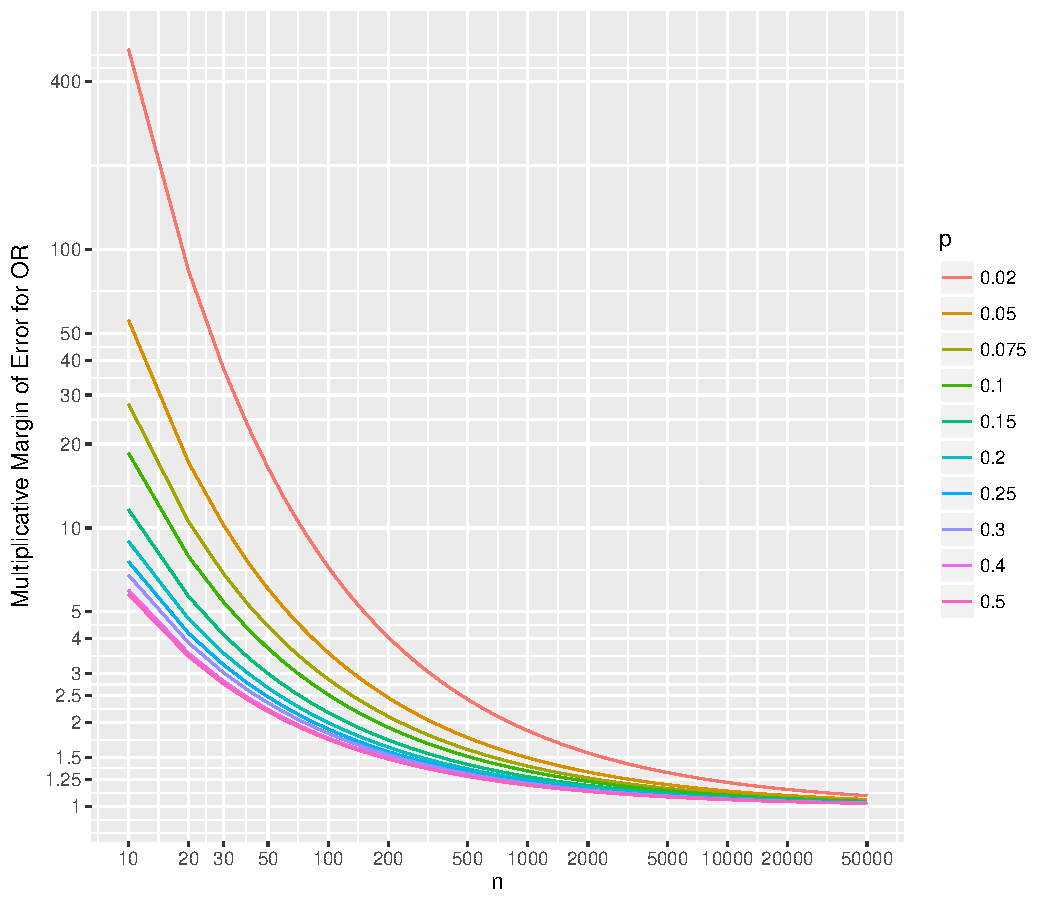
\includegraphics[width=\maxwidth]{prop-mmeor-1} }

\caption[Multiplicative margin of error for odds ratios]{Multiplicative margin of error related to 0.95 confidence limits of an odds ratio, for varying $n$ and $p$ (different curves), assuming the unknown true probability in each group is no lower than $p$}\label{fig:prop-mmeor}
\end{figure}
\end{Schunk}


\section{Comprehensive example}

\subsection{Study Description}
\bi
  \item Consider patients who will undergo coronary artery bypass graft surgery (CABG)
  \item Mortality risk associated with open heart surgery
  \item Study question: Do emergency cases have a surgical mortality that is different from that of non-emergency cases?
  \item Population probabilities
  \bi
    \item $p_1$: Probability of death in patients with emergency priority
    \item $p_2$: Probability of death in patients with non-emergency priority
  \ei
  \item Statistical hypotheses
  \bi
  \item $H_0: p_1 = p_2$ (or $\textrm{OR} = 1$)
  \item $H_1: p_1 \neq p_2$ (or $\textrm{OR} \neq 1$)
  \ei
\ei

\subsection{Power and Sample Size}

\bi
  \item Prior research shows that just over $0.1$ of surgeries end in death
  \item Researchers want to be able to detect a 3 fold increase in risk
  \item For every 1 emergency priority, expect to see 10 non-emergency
  \item $p_1 = 0.3$, $p_2 = 0.1$, $\alpha = 0.05$, and $\textrm{power} = 0.90$
  \item Calculate sample sizes using the PS software for these values and other combinations of $p_1$ and $p_2$
\ei

\begin{table}[!hbp]
 \begin{center}
 \begin{tabular}{lcccc} \hline\hline
$(p_1, p_2)$ &\boldmath$(0.3, 0.1)$&$(0.4, 0.2)$&$(0.03, 0.01)$&$(0.7, 0.9)$ \\ 
$n_1$  &\boldmath$40$&$56$&$589$&$40$ \\ 
$n_2$  &\boldmath$400$&$560$&$5890$&$400$ \\ \hline \hline
\end{tabular}
\end{center}
\end{table}
Check PS calculations against the \R\ \Co{Hmisc} package's
\Co{bsamsize} function.
\begin{Schunk}
\begin{Sinput}
round(bsamsize(.3, .1, fraction=1/11, power=.9))
\end{Sinput}
\begin{Soutput}
 n1  n2 
 40 399 
\end{Soutput}
\begin{Sinput}
round(bsamsize(.4, .2, fraction=1/11, power=.9))
\end{Sinput}
\begin{Soutput}
 n1  n2 
 56 561 
\end{Soutput}
\begin{Sinput}
round(bsamsize(.7, .9, fraction=1/11, power=.9))
\end{Sinput}
\begin{Soutput}
 n1  n2 
 40 399 
\end{Soutput}
\end{Schunk}

\subsection{Collected Data}

In-hospital mortality figures for emergency surgery and other surgery

\begin{table}[!hbp]
 \begin{center}
 \begin{tabular}{l|cc}
 & \multicolumn{2}{|c}{Discharge Status} \\
Surgical Priority& Dead& Alive \\ \hline
Emergency&$6$&$ 19$\\
Other&$11$&$100$\\
\end{tabular}
\end{center}
\end{table}

\bi
\item $\hat{p}_1 = \frac{6}{25} = 0.24$
\item $\hat{p}_2 = \frac{11}{111} = 0.10$
\ei

\subsection{Statistical Test}
\begin{Schunk}
\begin{Sinput}
n1 <- 25;     n2 <- 111
p1 <- 6 / n1; p2 <- 11 / n2
or <- p1 / (1 - p1) / (p2 / (1 - p2))
or
\end{Sinput}
\begin{Soutput}
[1] 2.870813
\end{Soutput}
\begin{Sinput}
# Standard error of log odds ratio:
selor <- sqrt(1 / (n1 * p1 * (1 - p1)) + 1 / (n2 * p2 * (1 - p2)))
# Get 0.95 confidence limits
cls <- exp(log(or) + c(-1, 1) * qnorm(0.975) * selor)
cls
\end{Sinput}
\begin{Soutput}
[1] 0.946971 8.703085
\end{Soutput}
\begin{Sinput}
tcls <- paste0(round(or, 2), ' (0.95 CI: [', round(cls[1], 2),
               ', ', round(cls[2], 2), '])')
# Multiplying a constant by the vector -1, 1 does +/-
x <- matrix(c(6, 19, 11, 100), nrow=2, byrow=TRUE)
x
\end{Sinput}
\begin{Soutput}
     [,1] [,2]
[1,]    6   19
[2,]   11  100
\end{Soutput}
\begin{Sinput}
chisq.test(x, correct=FALSE)
\end{Sinput}
\begin{Soutput}

	Pearson's Chi-squared test

data:  x
X-squared = 3.7037, df = 1, p-value = 0.05429
\end{Soutput}
\end{Schunk}
Ignore the warning about the $\chi^2$ approximation.
\bi
\item Interpretation
 \bi
 \item Compare odds of death in the emergency group
   $\left(\frac{\hat{p}_1}{1-\hat{p}_1}\right)$ to odds of death in
   non-emergency group  $\left(\frac{\hat{p}_2}{1-\hat{p}_2}\right)$ 
 \item Emergency cases have 2.87 (0.95 CI: [0.95, 8.7]) fold
   increased odds times of death during surgery compared to
   non-emergency cases. 
 \ei
\ei

\subsubsection{Fisher's Exact Test}

Observed marginal totals from emergency surgery dataset \\
\begin{tabular}{l|c|c|c} 
\multicolumn{1}{l}{} & \multicolumn{1}{c}{Dead} & \multicolumn{1}{l}{Alive} \\ \cline{2-3}
Emergency & $a$ & $b$ & $25$ \\ \cline{2-3}
Other & $c$ & $d$ &  $111$ \\ \cline{2-3}
\multicolumn{1}{l}{} & \multicolumn{1}{c}{$17$} & \multicolumn{1}{c}{$119$} & \multicolumn{1}{c}{$136$}
\end{tabular}

\bi
\item With fixed marginal totals, there are 18 possible tables ($a = 0, 1, \ldots 17$)
\item Can calculated probability of each of these tables
\bi
\item $p$-value: Probability of observing data as extreme or more extreme than we collected in this experiment
\ei
\item Exact test: $p$-value can be calculated ``exactly'' (not using the Chi-squared distribution to approximate the $p$-value)
\\
\begin{Schunk}
\begin{Sinput}
fisher.test(x)
\end{Sinput}
\begin{Soutput}

	Fisher's Exact Test for Count Data

data:  x
p-value = 0.08706
alternative hypothesis: true odds ratio is not equal to 1
95 percent confidence interval:
 0.7674155 9.6831351
sample estimates:
odds ratio 
  2.843047 
\end{Soutput}
\end{Schunk}
Note that the odds ratio from Fisher's test is a conditional maximum
likelihood estimate, which differs from the unconditional maximum
likelihood estimate we obtained earlier.
\item Fisher's test more conservative than Pearson's $\chi^2$ test
  (larger $P$-value) 
\ei

